\documentclass{article}
\usepackage{amsmath}
\usepackage{graphicx}
\usepackage{enumitem}
\usepackage{hyperref}
\usepackage[margin=1in]{geometry}

\title{XAI Techniques Cheatsheet}
\author{Yvo Keller}
\date{\today}

\begin{document}
\maketitle

\section{Tabular Methods}

\subsection{Shapley Values}

\subsubsection{Overview}
Shapley values provide a way to fairly distribute the prediction among features by considering all possible feature combinations.

\subsubsection{Key Formula}
The Shapley value for feature $i$ is:
\begin{equation}
    \phi_i(x) = \sum_{S \subseteq N \backslash\{i\}} \frac{|S|!\times(|N|-|S|-1)!}{|N|!}\left(f_\theta(S \cup\{i\})-f_\theta(S)\right)
\end{equation}

where:
\begin{itemize}
    \item $N$ is the set of all features
    \item $S$ is a subset of features excluding feature $i$
    \item $f_\theta$ is the model prediction
    \item $|S|$ is the size of subset $S$
    \item $|N|$ is the total number of features
\end{itemize}

\subsubsection{Calculation Process}
\begin{enumerate}
    \item Select an instance to explain
    \item For each feature:
    \begin{enumerate}
        \item Generate all possible feature coalitions excluding the target feature
        \item For each coalition:
        \begin{enumerate}
            \item Calculate model prediction with and without target feature
            \item Compute marginal contribution
            \item Weight contribution by coalition size
        \end{enumerate}
        \item Sum weighted contributions
    \end{enumerate}
    \item Average contributions over all permutations
\end{enumerate}

\subsubsection{Properties}
\begin{itemize}
    \item \textbf{Efficiency}: Sum of Shapley values equals model output minus baseline
    \item \textbf{Symmetry}: Equal contribution features receive equal Shapley values
    \item \textbf{Dummy}: Features with no marginal contribution get zero Shapley value
    \item \textbf{Additivity}: Values can be computed independently and summed
\end{itemize}

\subsubsection{Intuitive Example: Ice Cream Shop}
Let's understand Shapley values through a practical example of predicting ice cream sales.

\paragraph{Setup}
Consider a model predicting daily ice cream sales with features:
\begin{itemize}
    \item $x_1$ = Day of the week
    \item $x_2$ = Number of flights arriving
    \item $x_3$ = Temperature
    \item $x_4$ = Total opening hours
\end{itemize}

\paragraph{Calculation Process}
To calculate the Shapley value for temperature ($x_3$):

\begin{enumerate}
    \item \textbf{Select a sample}: Choose a specific day's data point
    \item \textbf{Choose baseline}: Select a reference point (usually average values)
    \item \textbf{Generate permutation}: e.g., $(x_4, x_1, x_3, x_2)$
    \item \textbf{Calculate marginal contributions}:
    \begin{itemize}
        \item Start with baseline prediction: $f_\text{base}$
        \item Add features one by one:
            \begin{align*}
                &f(x_4) \\
                &f(x_4, x_1) \\
                &f(x_4, x_1, x_3) \leftarrow \text{Temperature added here} \\
                &f(x_4, x_1, x_3, x_2)
            \end{align*}
        \item Temperature's contribution = $f(x_4, x_1, x_3) - f(x_4, x_1)$
    \end{itemize}
    \item \textbf{Repeat}: Do this for multiple permutations
    \item \textbf{Average}: The Shapley value is the average contribution across permutations
\end{enumerate}

\paragraph{Interpretation}
The final Shapley value for temperature tells us:
\begin{itemize}
    \item Positive value: Higher temperatures increase ice cream sales
    \item Negative value: Higher temperatures decrease sales
    \item Magnitude: Size of temperature's impact on the prediction
\end{itemize}

\subsubsection{Monte Carlo Approximation}
For large feature sets, exact computation becomes infeasible. Monte Carlo approximation:
\begin{enumerate}
    \item Sample random feature permutations
    \item Calculate marginal contributions for each permutation
    \item Average results over all samples
\end{enumerate}

\subsubsection{SHAP Summary Plot (Beeswarm)}
\begin{figure}[h]
    \centering
    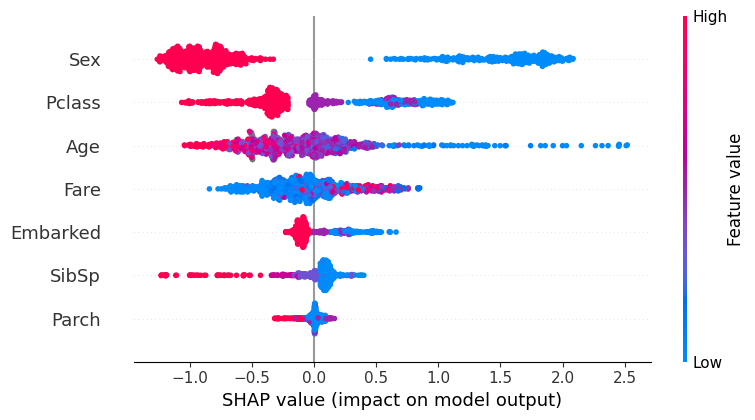
\includegraphics[width=0.8\textwidth]{resources/images/bee_swarm.png}
    \caption{SHAP Summary Plot showing feature importance and impact distribution}
    \label{fig:shap_summary}
\end{figure}

\paragraph{How to Read the Plot}
\begin{itemize}
    \item \textbf{Feature Ranking}: Features are ordered by importance from top to bottom
    \item \textbf{Impact}: The x-axis shows SHAP values (impact on model output)
        \begin{itemize}
            \item Positive values (right) indicate increased likelihood of the prediction
            \item Negative values (left) indicate decreased likelihood
            \item Magnitude shows strength of impact
        \end{itemize}
    \item \textbf{Distribution}: Each dot represents one instance in the dataset
    \item \textbf{Color Coding}:
        \begin{itemize}
            \item Red indicates high feature values
            \item Blue indicates low feature values
            \item Color gradient shows the feature value spectrum
        \end{itemize}
    \item \textbf{Spread}: Horizontal spread shows the distribution of impacts across instances
\end{itemize}

\paragraph{Example Interpretation}
Using the plot above:
\begin{itemize}
    \item \textbf{Sex}: Shows strong impact with clear separation between categories
    \item \textbf{Pclass}: Passenger class has significant influence, with higher classes (blue) generally having positive impact
    \item \textbf{Age}: Shows varied effects across different age groups
    \item \textbf{Fare}: Demonstrates complex relationships with both positive and negative impacts
    \item \textbf{Embarked}: Port of embarkation shows moderate influence
    \item \textbf{SibSp \& Parch}: Family-related features show smaller but notable effects
\end{itemize}

\subsection{Partial Dependence Plots (PDP)}

\subsubsection{Overview}
PDPs show how a feature affects predictions on average, while marginalizing over all other features.

\begin{figure}[h]
    \centering
    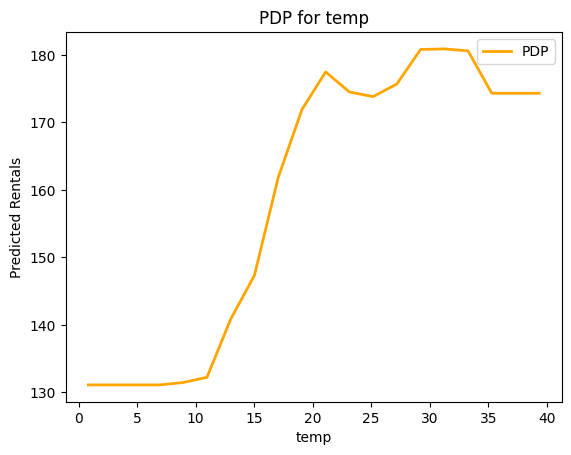
\includegraphics[width=0.8\textwidth]{images/pdp.png}
    \caption{Example of a Partial Dependence Plot (PDP)}
    \label{fig:pdp}
\end{figure}

\subsubsection{Intuitive Example}
Consider our ice cream sales model:
\begin{itemize}
    \item To create a PDP for temperature:
    \begin{enumerate}
        \item Pick a temperature value (e.g., 25°C)
        \item For every data point, set temperature to 25°C
        \item Get model predictions for all these modified points
        \item Average these predictions
        \item Repeat for different temperature values
        \item Plot temperature vs. average predictions
    \end{enumerate}
\end{itemize}

\subsubsection{Interpretation}
\begin{itemize}
    \item Slope shows relationship strength
    \item Shape reveals non-linear effects
    \item Flat regions indicate no impact
    \item Limitations: Can miss feature interactions
\end{itemize}

\subsection{Individual Conditional Expectation (ICE)}

\subsubsection{Overview}
ICE plots extend PDPs by showing how predictions change for individual instances, revealing heterogeneous effects hidden by PDPs.

\begin{figure}[h]
    \centering
    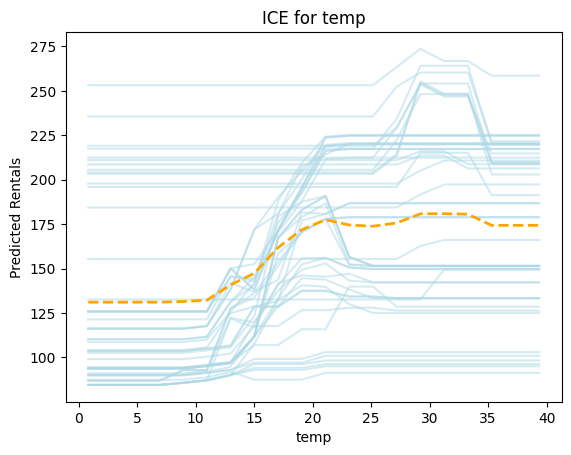
\includegraphics[width=0.8\textwidth]{images/ice.png}
    \caption{Example of Individual Conditional Expectation (ICE) plots}
    \label{fig:ice}
\end{figure}

\subsubsection{Intuitive Example}
Using our ice cream model:
\begin{itemize}
    \item For each individual day in our dataset:
    \begin{enumerate}
        \item Keep all features fixed except temperature
        \item Vary temperature across its range
        \item Plot prediction line for this specific day
    \end{enumerate}
    \item Result: Multiple lines, one per instance
    \item PDP would be the average of these lines
\end{itemize}

\subsubsection{Key Insights}
\begin{itemize}
    \item Diverging lines suggest feature interactions
    \item Parallel lines indicate consistent effects
    \item Crossing lines show complex relationships
    \item More informative than PDP alone
\end{itemize}

\subsubsection{When to Use}
\begin{itemize}
    \item Feature interaction analysis
    \item Detecting heterogeneous effects
    \item Model behavior validation
    \item Identifying outlier instances
\end{itemize}

\end{document} 